\localauthor{Stefanie Gürster}
\subsection{Benutzerfluss}
Im Folgenden werden funktionale Aussagen über die Benutzeroberfläche, mithilfe eines Benutzerflussdiagramms, getroffen.

\begin{figure}[H]
	\centering
	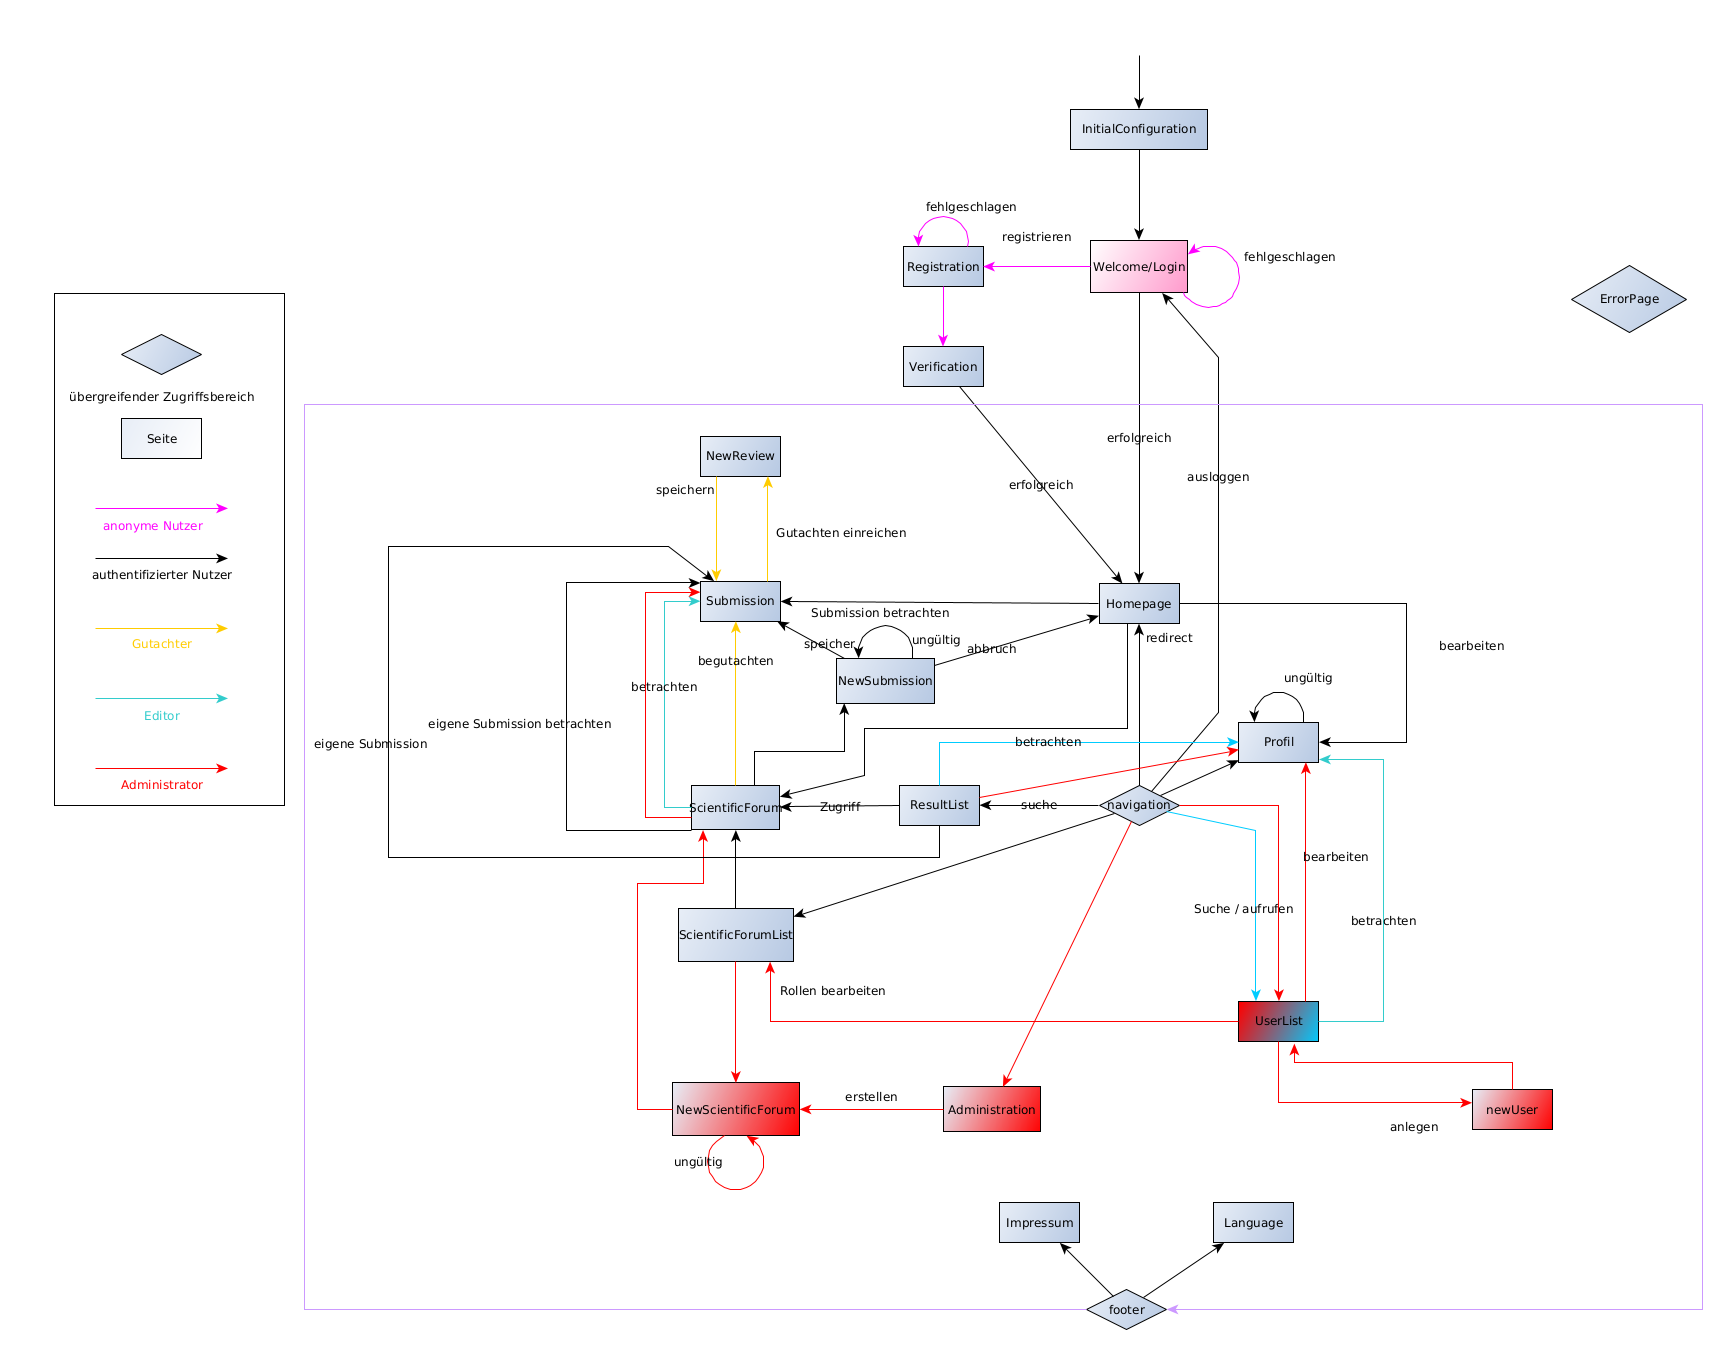
\includegraphics[width=\linewidth]{graphics/benutzerFlussyEd-png}
	\caption{Analyse der Navigationsstruktur}
	\label{fig:benutzerfluss}
\end{figure}

Die sich im Diagramm in Abbildung \ref{fig:benutzerfluss} befindlichen Rauten stellen Header (Navigationsleiste) und Footer dar.
Hierbei wird jedoch wie folgt unterschieden: Der Header ist nur für \hyperref[mkrit:angemeldet]{authentifizierte Nutzer} zugänglich,
d.h. dieser erscheint erst nach einem erfolgreichen Login und verschwindet nach dem Logout wieder.
Der Footer hingegen ist von jeder Seite der Applikation zugänglich und somit immer sichtbar.

Im Diagramm werden \hyperref[mkrit:admin]{Administratoren}, \hyperref[mkrit:editor]{Editoren}, \hyperref[mkrit:gutachter]{Gutachter} und \hyperref[mkrit:angemeldet]{normale Nutzende} unter dem allgemeinen Begriff
authentifizierte Nutzer betrachtet.
Sind die Verbindungspfeile nicht schwarz, sondern andersfarbig dargestellt, so besitzen auch nur die
dargestellten Benutzergruppen ein Zugriffsrecht oder das Recht auf eine Aktion. (Administratoren sind von dieser Regelung
ausgeschlossen.)

Zur Übersichtlichkeit wurde auf die Navigation zur Errorpage verzichtet.

\subsection{Wireframe}

Die Grundstruktur der Ansichten wird in Abbildung \ref{fig:wireframe} abgebildet, welche sich auch in den folgenden Mockups in Abbildung \ref{fig:homepageMockup} und in Abbildung \ref{fig:submission} wiederspiegelt.
Inhalte mit gestrichelten Linen sind dabei nicht immer in jeder Ansicht sichtbar.

\begin{figure}[H]
	\centering
	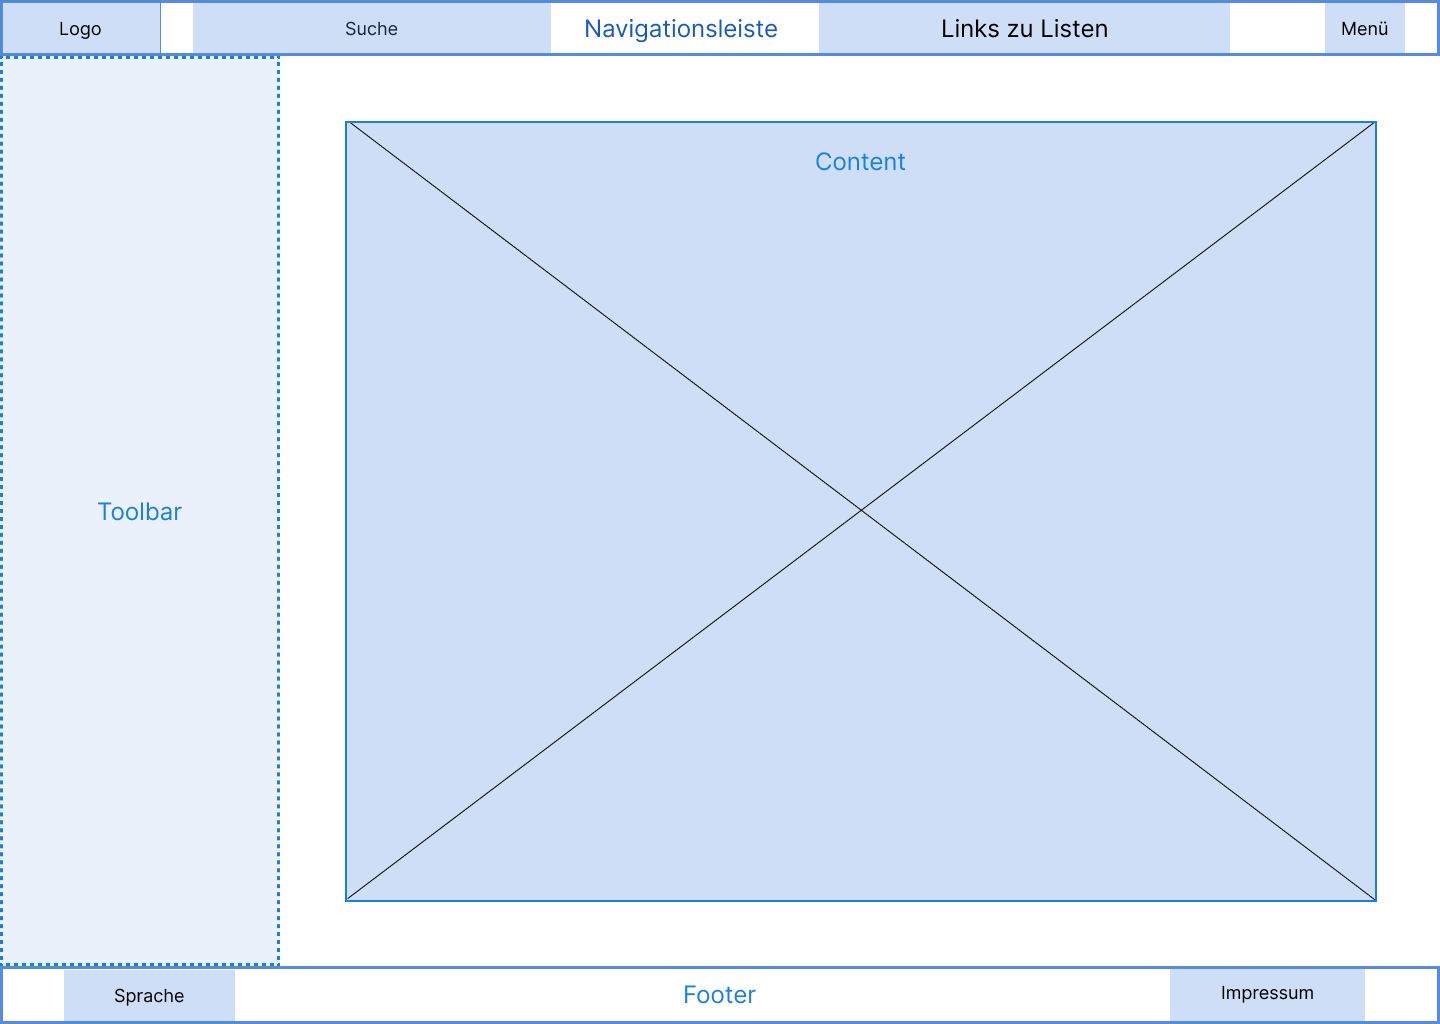
\includegraphics[width=0.85\linewidth]{graphics/Wireframe-png}
	\caption{Grundstruktur der Ansichten}
	\label{fig:wireframe}
\end{figure}

\subsection{Mockups}

Folgende Bilder zeigen einen Prototyp der Anwendung.
Dargestellt sind zwei Ausschnitte aus Schlüsselfunktionen der Webanwendung.

Die Startseite in Abbildung \ref{fig:homepageMockup} ist auf die Rolle eines \hyperref[mkrit:editor]{Editors} zugeschnitten, wobei dieser auch einige
Gutachten bearbeitet und somit auch die Rolle des \hyperref[mkrit:gutachter]{Gutachters} für einige Einreichungen bekleidet.
Je nach ausgewähltem Reiter erscheinen entweder eigene, zu begutachtende Einreichungen oder Einreichungen die in eigener editorialer Verantwortung liegen.

Die Übersichtsseite der Einreichung, die Submission Seite, in Abbildung \ref{fig:submission} ist ebenfalls auf die Rolle eines \hyperref[mkrit:editor]{Editors} ausgelegt.
Ihm steht im Gegensatz zu einem \hyperref[mkrit:angemeldet]{normalen Nutzer}, welcher keine andere Rolle bekleidet, eine Toolbar zur Verfügung.
Mithilfe dieser kann er Gutachter verwalten, einem anderen \hyperref[mkrit:editor]{Editor} die Verwaltung der Einreichung übertragen oder eine Revision anfordern.


\subsubsection{Startseite}

\begin{figure}[H]
	\centering
	
\includegraphics[width=0.85\linewidth]{graphics/Homepage-png}
	\caption{Übersicht auf einer Startseite}
	\label{fig:homepageMockup}
\end{figure}

\subsubsection{Submission}

\begin{figure}[H]
	\centering
	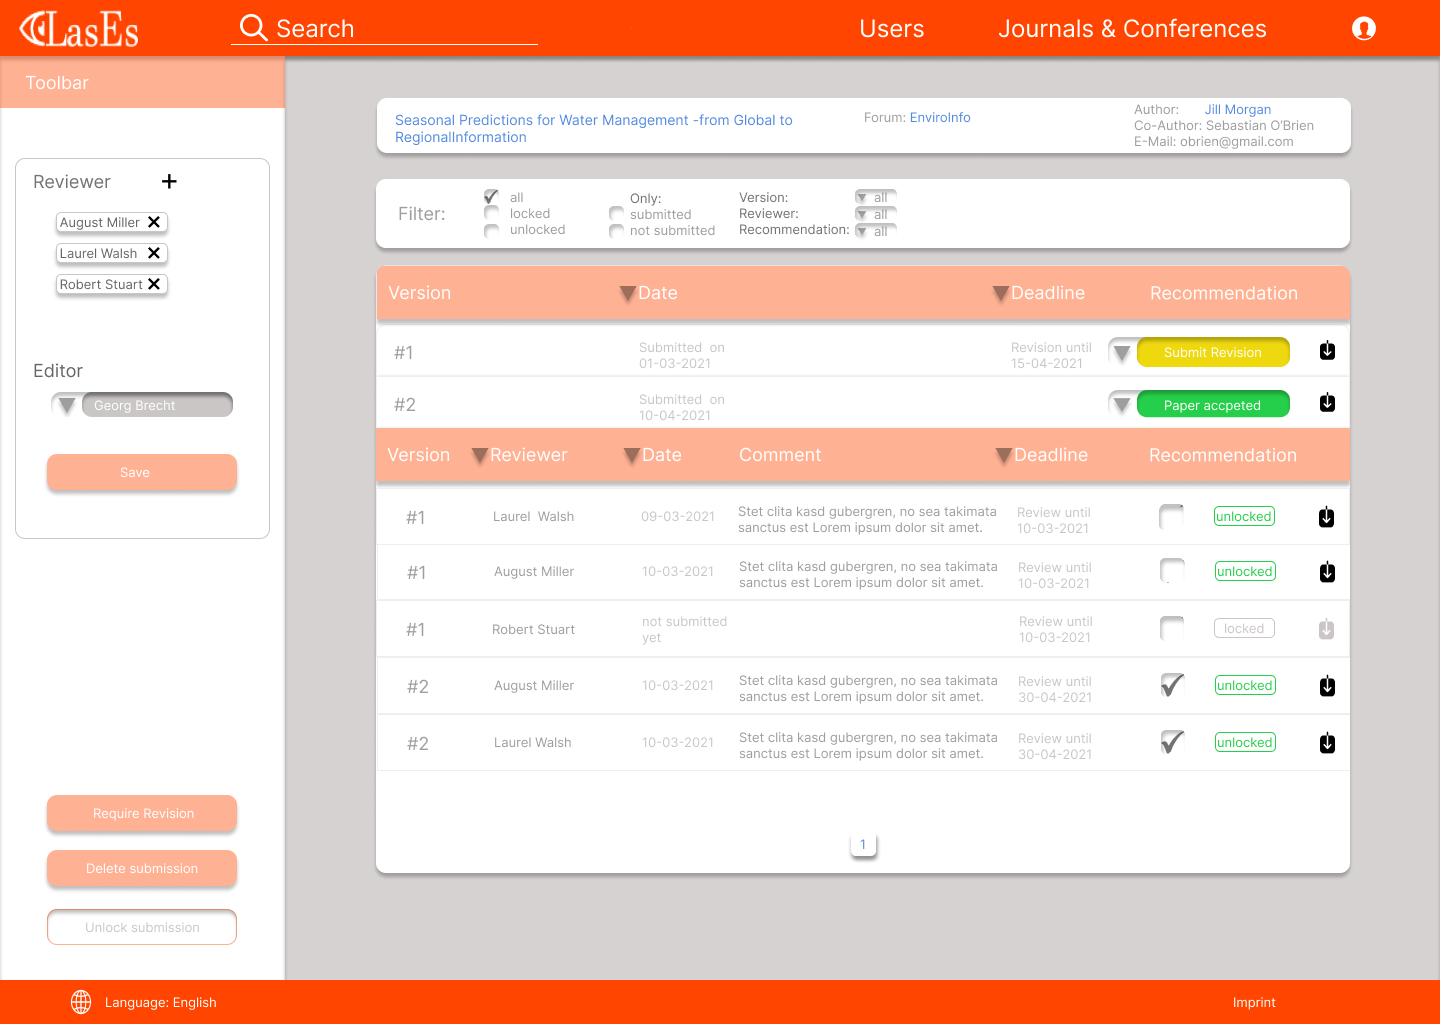
\includegraphics[width=0.85\linewidth]{graphics/Submission-png}
	\caption{Verwaltung einer Einreichung}
	\label{fig:submission}
\end{figure}